\begin{figure}[h!]
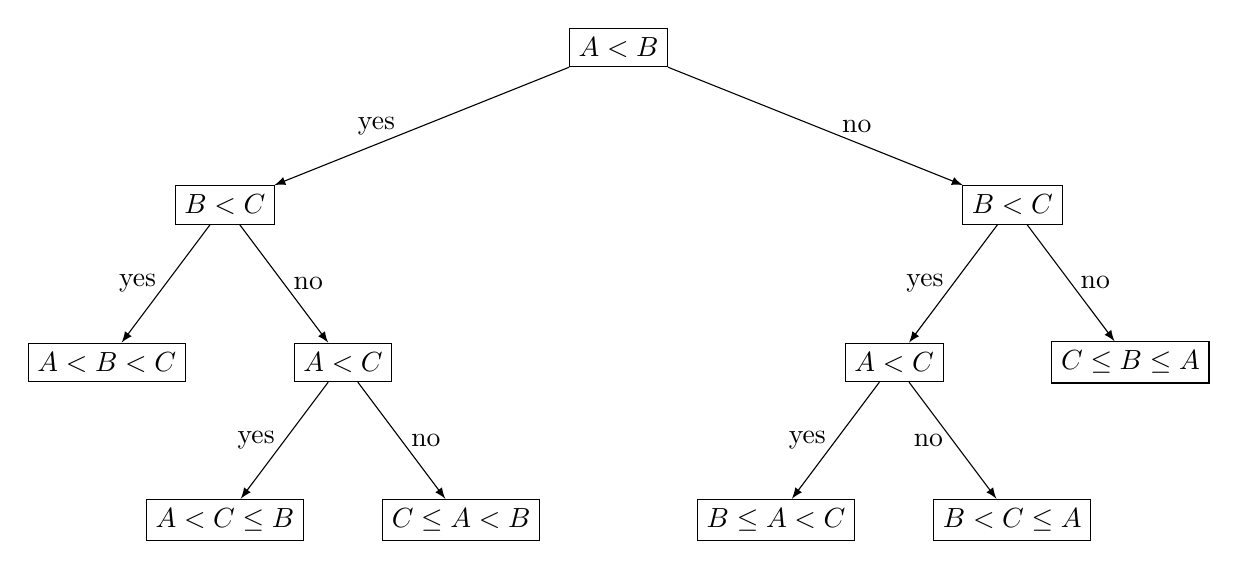
\begin{tikzpicture}[edge from parent/.style={draw,-latex},
level distance=2cm,
level 1/.style={sibling distance=10cm},
level 2/.style={sibling distance=3cm}]
\tikzstyle{every node}=[rectangle,draw]    
\node (Root) {$A < B$}
child {
    node {$B < C$}    
    child { 
        node {$A < B < C$} 
        edge from parent node[left,draw=none] {yes}
    }
    child { 
        node {$A < C$} 
        child {
            node {$A < C \leq B$}
            edge from parent node[left,draw=none] {yes}
        }
        child {
            node {$C \leq A < B$}
            edge from parent node[right,draw=none] {no}
        }
        edge from parent node[right,draw=none] {no}
    }
    edge from parent node[left,draw=none] {yes $\;$}
}
child {
    node {$B < C$}
    child { 
        node {$A < C$}     
        child {
            node {$B \leq A < C$}
            edge from parent node[left,draw=none] {yes}
        }   
        child {
            node {$B < C \leq A$}
            edge from parent node[left,draw=none] {no}
        }     
        edge from parent node[left,draw=none] {yes}
    }
    child { 
        node {$C \leq B \leq A$} 
        edge from parent node[right,draw=none] {no}
    }
    edge from parent node[right,draw=none] { $\;$ no}
};
\end{tikzpicture}
\caption{A decision tree for sorting three values.}
\label{fig:sortingtree}
\end{figure}
